\section{Methodology}\label{sec:method}
In this section, we discuss the problem of some methods (e.g., \fedavg) in cross-device FL, and then propose our predict-observe framework and a method \fedeve to deal with it.  

\subsection{Typical Federated Learning Setup}\label{sec:fedavg}
Federated learning, as described by \citet{mcmahan2017communication}, involves utilizing multiple clients and a central server to optimize the overall learning objective. The goal is to minimize the following objective function:
\begin{equation}
\label{eq:obj}
\min_w~f(w) = \sum_{k=1}^N p_k F_k(w)= \mathbb{E}_k [F_k(w)],
% %\vspace{-1mm}
\end{equation}
where $N$ is the number of clients, $p_k\geq 0$, and $\sum_k p_k$=$1$. In general, the global objective is the expectation of the local objective over different data distributions $\mathcal{D}_k$, i.e., $F_k(w) = \mathbb{E}_{x_k \sim \mathcal{D}_k}{f_k(w;x_k)}$, with $n_k$ samples on each client $k$ and weighted by $p_k$. We set $p_k$=$\frac{n_k}{n}$, where $n$= $\sum_k n_k$ is the total number of data points. In deep learning setting, $F_k(w)$ is often non-convex.
A common approach to solve the objective (\ref{eq:obj}) in federated settings is \fedavg  \citep{mcmahan2017communication}. For example, in cross-device FL, a small subset $\mathcal{S}_t$ ($|\mathcal{S}_t| \ll N$) of the total clients are selected at each round (ideally randomly, but possibly biased in practice), and then the server broadcasts its global model to the selected client. In parallel, each of the selected clients runs SGD on their own loss function  $F_k\left(\cdot\right)$ for $E$ number of epochs, and sends the resulting model to the server. The server then updates its global model as the average of these local models and repeats this process until convergence. 
One problem of FL is the non-iid data across clients, which can bring about ``client drift" in the updates of each client, resulting in slow and unstable convergence \citep{karimireddy2021scaffold}. Despite efforts to address the problem of client drift \citep{karimireddy2021scaffold,li2020federated,reddi2020adaptive}, there is a lack of research on the issue of period drift, i.e. the data distribution of selected clients at each round may differ from the overall data distribution of all clients. Period drift along with client drift can greatly impact the convergence of the learning process in FL, thus we propose a predict-observe framework to deal with them.

\subsection{The Concept of Drift} \label{sec:impact}
In contrast to conventional distributed optimization, federated learning possesses distinct characteristics, such as client sampling, multiple local epochs, and non-iid data distribution. These attributes may lead to a drift in the updates of global model, resulting in suboptimal performance. This drift can be thought of as a noise term that is added to the true optimization states during the optimization process. Thus, we can make the definition of period drift and client drift as:

\begin{definition}[Period Drift and Client Drift]\label{def:drifts}
In federated learning, two types of drift arise from data heterogeneity:
\begin{itemize}[leftmargin=*]
    \item \textbf{Period Drift:} The deviation when the data distribution of selected clients differs from the overall distribution. Formally:
    \begin{equation}
        \text{Period Drift} := \mathbb{E}_{\mathcal{S}_t} \left[ \left\| \frac{1}{|\mathcal{S}_t|} \sum_{k \in \mathcal{S}_t} \nabla F_k(w) - \nabla f(w) \right\|^2 \right],
    \end{equation}
    where $\mathbb{E}_{\mathcal{S}_t}$ is the expectation over client sampling, $\mathcal{S}_t$ is the subset of clients selected at round $t$, $\nabla F_k(w)$ is the gradient of client $k$'s objective, and $\nabla f(w)$ is the gradient of the global objective.
    
    \item \textbf{Client Drift:} The deviation when the averaged optima of local objectives does not align with the optimum of the averaged objective. Formally:
    \begin{equation}
        \text{Client Drift} := \mathbb{E}_{k \in \mathcal{S}_t} \left[ \left\| \nabla F_k(w_k^*) - \nabla F_k(w_{\mathcal{S}_t}^*) \right\|^2 \right],
    \end{equation}
    where $w_k^*$ is the local optimum for client $k$ and $w_{\mathcal{S}_t}^*$ is the optimum for the selected clients' averaged objective.\looseness-1
\end{itemize}
These drifts are conceptually independent but together affect model convergence and performance. See Appendix~\ref{appdx:concept} for detailed discussion.
\end{definition}

\begin{assumption}\label{assum:drift}
   \textit{The aggregated model parameters on the server $w_{server}$, can be represented as the sum of the optimal parameters $w^*$ and a drift (noise) that follows a normal distribution ${w}_{drift} \sim \mathcal{N}(0,\sigma_{drift}^2)$:}
   \begin{equation}\label{eq:drift}
      {w}_{server}={w}^*+{w}_{drift}\leftarrow noise,
   \end{equation}
\end{assumption}
% \begin{equation}\label{eq:drift}
%    {w}_{server}={w}^*+{w}_{drift}\leftarrow noise,
% \end{equation}
where $w^*$ represents the optimal parameters obtained through the use of stochastic gradient descent (SGD), $w_{drift}$ represents the noise term caused by factors such as client sampling, multiple local epochs, and non-iid data distribution that we assume a normal distribution, and $w_{server}$ represents the aggregated model parameters also follows a normal distribution ${w}_{server} \sim \mathcal{N}(w^*,\sigma_{drift}^2)$, with the expectation of the aggregate model parameters being equal to the optimal parameters, i.e. $\mathbb{E}[{w}_{server}]={w}^*$. Note that the assumption of Gaussian-like noise is natural, and its justification can be found in Appendix \ref{sec:assum1_just}.

% In order to investigate the effect of the deviation on performance in FL, we utilize a regression optimization objective as in previous studies, such as \citep{zhang2019lookahead} and \citep{wu2018understanding}:
%   $$
%   \hat{\mathcal{L}}({w})=\frac{1}{2}({w}+{w}_{drift})^T {A}({w}+{w}_{drift}),
%   $$
% where ${w}_{drift} \sim \mathcal{N}(0,\sigma^2)$ is the drift caused by the characteristics of FL. Therefore, the generalization error can be formulated as:
% \begin{equation*}
%    \small
%    \begin{aligned}
%       \mathcal{L}\left(w^{t}\right)&=\mathbb{E}\left[\hat{\mathcal{L}}\left(w^{t}\right)\right]=\frac{1}{2} \mathbb{E}\left[\sum_i a_i\left(w_i^{t^2}+\sigma_i^2\right)\right]\\
%       &=\frac{1}{2} \sum_i a_i\left(\mathbb{E}\left[w_i^{t}\right]^2+\mathbb{V}\left[w_i^{t}\right]+\sigma_i^2\right).
%    \end{aligned}
% \end{equation*}
% In the context of FL, the generalization error can also be decomposed into three components: bias, variance, and noise. The noise component in this context is further influenced by factors such as client sampling, multiple local epochs, and non-iid data distribution, leading to a much larger overall generalization error compared to traditional stochastic gradient descent. Thus, our goal is to reduce the variance of drift $\sigma^2$ in order to improve both the convergence and performance of the model. By reducing the variance of drift, we can ensure that the updates made to the model are more consistent and accurate, leading to better overall performance. The subsequent section of this study aims to investigate the influence of drift on both the server and client side with respect to this noise component in federated learning.

\subsection{The Predict-observe Framework}
Initially, we establish the concept of period drift, represented by $Q_t$, and client drift, represented by $R_t$ at the $t$-th communication round. We first make an assumption of independence concerning the two types of drift, which states that the two drifts are independent of one another. This assumption allows us to more accurately analyze the impact of each drift on the model's performance and devise methods to mitigate their effects.
% \begin{assumption}\label{assum:wqr}
%    \textit{The period drift and client drift are independent of each other at each communication round and also independent to the initialization model parameters, that is $w_0 \perp Q_0 \perp Q_1 \perp \cdots Q_t \perp R_0 \perp R_1 \perp \cdots R_t$.}
% \end{assumption}

\begin{assumption}\label{assum:wqr}
   \textit{The initialization model parameters are independent of all period drifts $Q_t$ and client drifts $R_t$ at each communication round, that is $w_0 \perp Q_0, Q_1,\cdots, Q_t$ and $w_0 \perp R_0,  R_1,\cdots, R_t$.}
   \end{assumption}
The justification and limitation of this assumption can be found in Appendix \ref{sec:assum2_just}.
Since the clients participating in each round in cross-device FL is only a small fraction of all clients, 
% the data distribution of these clients $\mathcal{U}_t= \cup_{k \in \mathcal{S}_t}\mathcal{D}_k$ is the approximation of overall distribution. 
period drift can be attributed to the discrepancy that the objective of selected clients at each round does not align with the overall objective. Thus, an effective prediction of updates can potentially help reduce the period drift. As formulated in Equation (\ref{eq:drift}), we express the prediction of updates on the server as:
\begin{equation}\label{eq:predict}
   \hat{w}_{t+1}=g(w_{t})+Q_{t}, \quad Q_{t} \sim \mathcal{N}(0,\sigma_{Q_t}^2),
\end{equation}
where $\hat{w}_{t+1}$ is the prediction model of $(t+1)$-th round as the output of predcit function $g(\cdot)$ with the current model $w_{t}$ as input. It is noteworthy that the period drift at the $t$-th round is represented by $Q_{t}$, and just like the drift in assumption \ref{assum:drift}, it is assumed to follow a normal distribution $\mathcal{N}(0,\sigma_{Q_t}^2)$, characterized by a mean of zero and a variance of $\sigma_{Q_t}^2$. Client drift can be attributed to the phenomenon that the averaged optima of objectives does not align with the optima of averaged objectives. Thus, we consider the updates provided by these clients is a kind of observation of global updates. As formulated in Equation (\ref{eq:drift}), we express it as:
\begin{equation}\label{eq:observe}
\tilde{w}_{t+1} =h(\hat{w}_{t+1})+R_{t},\quad R_{t} \sim \mathcal{N}(0,\sigma_{R_t}^2),
\end{equation}
where $\tilde{w}_{t+1} $ is the model of $(t+1)$-th round as the output of observe function $h(\cdot)$ with the predict model $w_{t}$ as input. Also, the client drift at the $t$-th round is represented by $R_{t}$, and just like the drift in assumption \ref{assum:drift}, it is assumed to follow a normal distribution $\mathcal{N}(0,\sigma_{R_t}^2)$, characterized by a mean of zero and a variance of $\sigma_{R_t}^2$. It is clear that standard \fedavg is a special case since there is no prediction for server optimization, and it solely relies on the observations provided by clients.
Furthermore, the period drift, $Q_{t}$, and the client drift, $R_{t}$, are represented as noise terms that are incorporated into the prediction and observation functions. According to assumption (\ref{assum:wqr}), these drifts are independent of the current model states, and the lemma of independence noise is posited:
\begin{lemma}
   \label{lemma:independence_noise}
   \textit{(Independence of Noise). the noise present in the prediction and observation at each communication round is independent of the current model state, specifically, $w_t \perp Q_t$ and $w_t \perp R_t$.}
\end{lemma}
The complete proof of the independence of noise can be found in appendix \ref{appdx:noise}. 
The equations presented in equations \ref{eq:predict} and \ref{eq:observe} depict the prediction and observation of updates, respectively, taking into account both period drift and client drift. In order to reconcile the discrepancy between the prediction (including period drift) and observation (including client drift), a Bayesian filter is introduced to allow for compensation between the two sources of drift. The prior probability of $w_{t+1}$ is represented by $P(\hat{w}_{t+1})$, and by combining the observation $P(\tilde{w}_{t+1})$ and the likelihood $P(\tilde{w}_{t+1} \mid \hat{w}_{t+1})$, the posterior probability $P(w_{t+1} \mid\tilde{w}_{t+1})$ of $w_{t+1}$ can be calculated as the new model at the $(t+1)$-th round, as shown in Equation (\ref{eq:bayesian}).
\begin{equation}\label{eq:bayesian}
   \small
   \begin{aligned}
   P(\colorbox{green!10}{$w_{t+1}$})&:=P(\colorbox{red!10}{$\hat{w}_{t+1}$} \mid\colorbox{blue!10}{$\tilde{w}_{t+1} $})
   =\frac{P(\colorbox{blue!10}{$\tilde{w}_{t+1} $} \mid \colorbox{red!10}{$\hat{w}_{t+1}$}) P(\colorbox{red!10}{$\hat{w}_{t+1}$})}{P(\colorbox{blue!10}{$\tilde{w}_{t+1} $})}.
   \end{aligned}
\end{equation}
By utilizing the Bayesian filter in our predict-observe framework, an update mechanism is implemented that first performs prediction and then observes the predicted model state, as described in the following procedure:
\begin{equation}\label{eq:update}
   \small
   \begin{aligned}
   f_{w_t}^{+}(w) &\stackrel{\text {predict}}{\Longrightarrow} f_{\hat{w}_{t+1}}^{-}(w)=\int_{-\infty}^{+\infty} f_{Q_t}[w-f(v)] f_{w_t}^{+}(v) \mathrm{d} v\\ &\stackrel{\text {observe}}{\Longrightarrow} f_{w_{t+1}}^{+}(w)=\eta_t \cdot f_{R_t}\left[w_{t+1}-h(w)\right]
   \cdot f_{\hat{w}_{t+1}}^{-}(w),
   \end{aligned}
   \end{equation}
where $f_{w_t}^{+}(w)$ is the posterior probability of $w_{t}$, $f_{\hat{w}_{t+1}}^{-}(w)$ is the prior probability of $w_{t+1}$, $f_{Q_t}$ is the PDF of period drift, $f_{w_{t+1}}^{+}(w)$ is the posterior probability of $w_{t+1}$, $f_{R_t}$ is the PDF of client drift, and $\eta_t=\left\{\int_{-\infty}^{+\infty} f_{R_t}\left[\tilde{w}_{t+1}-h(\hat{w}_{t+1})\right] f_{\hat{w}_{t+1}}^{-}(w) \mathrm{d} w\right\}^{-1}$. By combining prediction and observation, the fused model can be estimated by taking the expectation of the posterior probability as follow:
\begin{equation}\label{eq:expectation}
   \hat{w}_{t+1}=E\left[f_{w_{t+1}}^{+}(w)\right]=\int_{-\infty}^{+\infty} w f_{w_{t+1}}^{+}(w) \mathrm{d} w.
   \end{equation}

\begin{theorem}\label{theorem:fused}
   \textit{Given assumption \ref{assum:drift} and lemma \ref{lemma:independence_noise}, the composite model will exhibit a diminished degree of variance in comparison to the individual variances of both period drift and client drift, and the mean will be a linear combination that is weighted by the variances:
\begin{equation}
   \begin{aligned}
   \mu_{\text {fused }}=\frac{\mu_1 \sigma_{R_t}^2+\mu_2 \hat{\sigma}^2_{t+1}}{\sigma_{R_t}^2}, \quad
   \sigma_{\text {fused }}^2=\frac{\hat{\sigma}^2_{t+1} \sigma_{R_t}^2}{\hat{\sigma}^2_{t+1}+\sigma_{R_t}^2},
   \end{aligned}
\end{equation}
where $\mu_1,\mu_2,\mu_{fused}$ is the mean of prediction, observation and fused model, and $\hat{\sigma}^2_{t+1},\sigma_{R_t}^2,\sigma_{fused}^2$ is the variance of prediction, client drift and fused model.}
\end{theorem}   
% \begin{figure}[hb]
%    \centering
%    \subfigure[Bayesian filter]{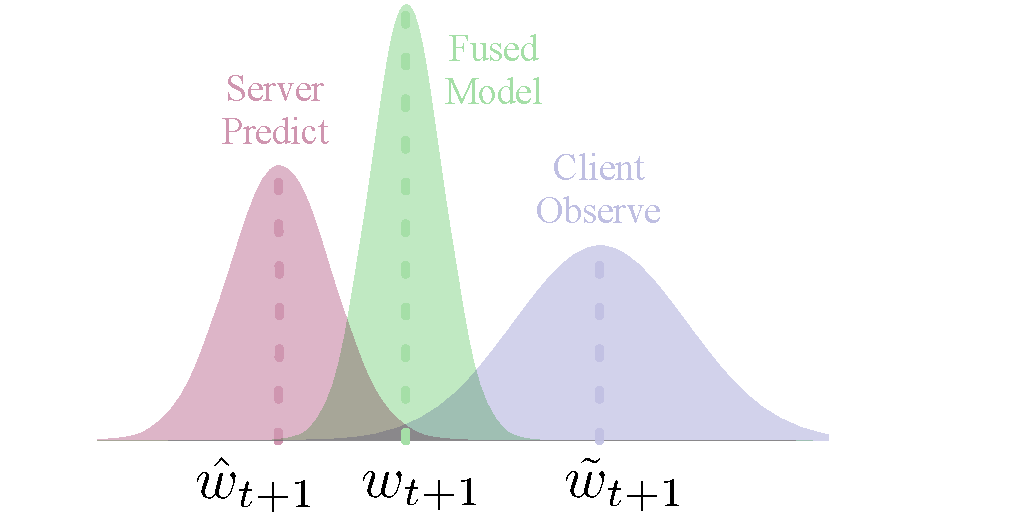
\includegraphics[width=0.49\linewidth]{filter.pdf}\label{fig:filter}}
%    \subfigure[\fedeve]{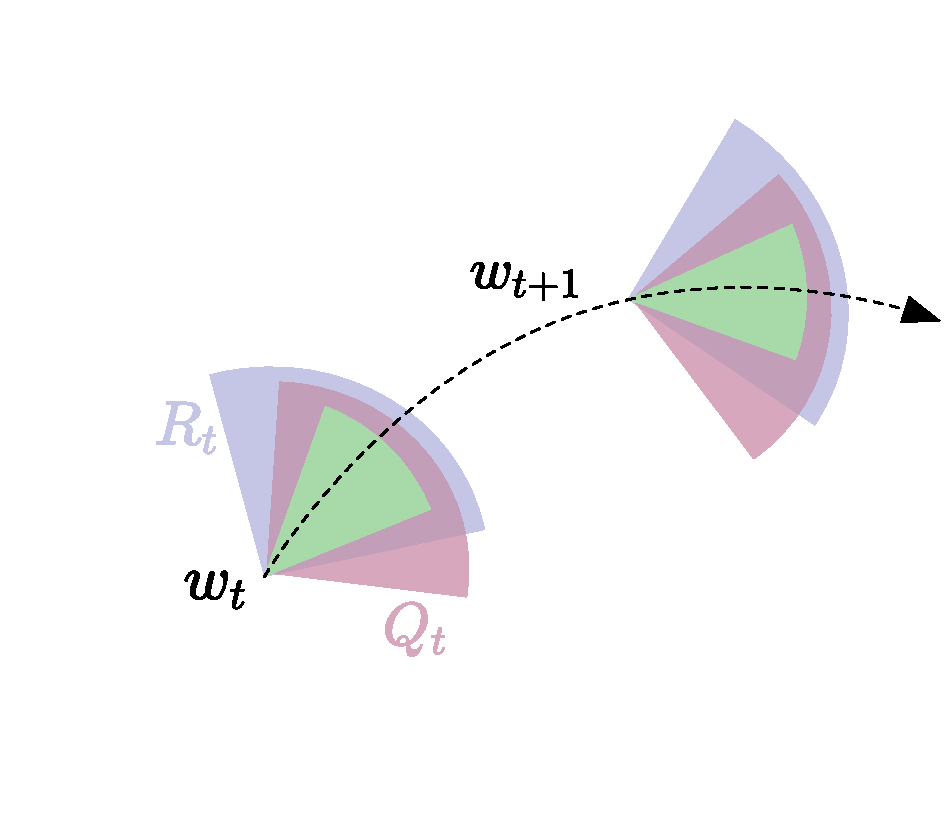
\includegraphics[width=0.49\linewidth]{fedeve1.pdf}\label{fig:algo}}
%    \caption{\small\textbf{Illustrations of the framework and \fedeve}.}
%    %\vspace{-4mm}
% \end{figure}
\begin{wrapfigure}{r}{0.55\textwidth}
   \vspace{-3mm}
   \centering
   \subfigure[Bayesian filter]{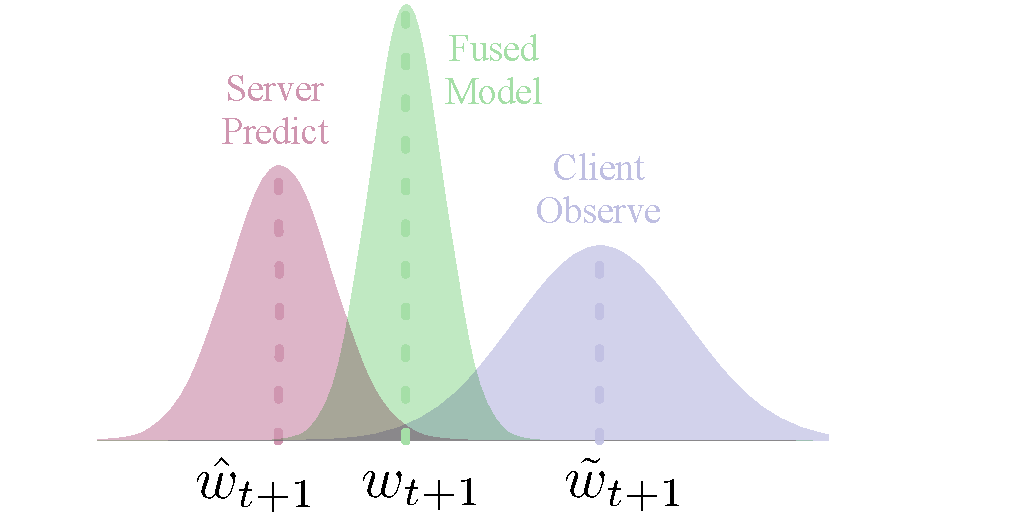
\includegraphics[width=0.49\linewidth]{filter.pdf}\label{fig:filter}}
   \subfigure[\fedeve]{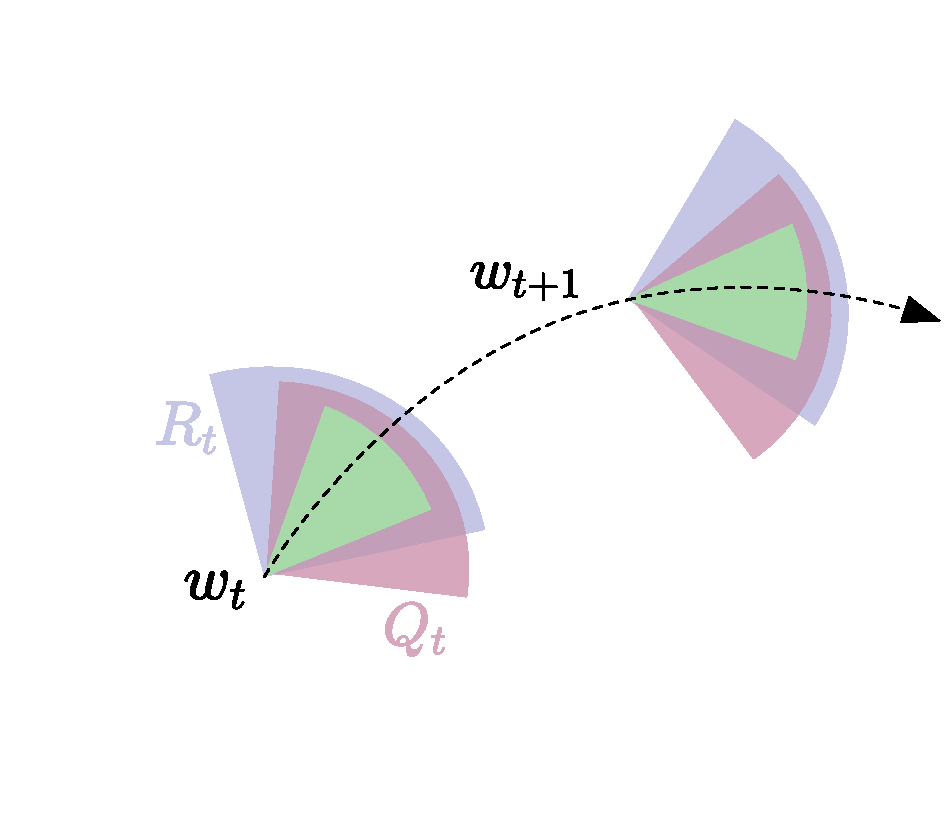
\includegraphics[width=0.49\linewidth]{fedeve1.pdf}\label{fig:algo}}
   \caption{\small\textbf{Illustrations of the framework and \fedeve}}
   \vspace{-3mm}
\end{wrapfigure}
The complete proof of the bayesian filter can be found in appendix \ref{appdx:bayesian}. The application of Bayesian filtering allows for the interaction of period drift and client drift to generate a new model, 
which is characterized by a reduced level of variance as compared to the individual variances of period drift and client drift, as depicted in Figure \ref{fig:filter}.
However, the computation of the new model is challenging due to the presence of infinite integrals in Equation (\ref{eq:expectation}) and $\eta_t$, as it is a general framework for any prediction and observation function. In the following section, we will propose a specialized method to facilitate the convergence of FL.


\subsection{The \fedeve Method}

The predict-observe framework has been proposed as a strategy for mitigating the challenges of period drift and client drift. However, it also raises some questions regarding the effective method of prediction and the variance associated with both period and client drift. In this section, we demonstrate that the utilization of momentum as a server optimization \citep{hsu2019measuring,reddi2020adaptive}, can serve as an effective prediction method. Furthermore, we present a method for estimating the variance of period drift and client drift. In the context of the predict-observe framework, we have adapted it to a specific setting where Nesterov momentum is employed as the prediction function $g(\cdot)$, and the observation function $h(\cdot)$ is the average of the models from the clients the same as \fedavg. We have reformulated \fedavg in an incremental form as the starting point of our approach.
\begin{equation}\label{eq:client_update}
   \small
   \begin{aligned}
      w_{t+1}&=\sum_{k \in \mathcal{S}_t}p_k w^k_t=w_t-\sum_{k \in \mathcal{S}_t}p_k \left(w_t-w^k_t\right)\\
      &=w_t-\sum_{k \in \mathcal{S}_t}p_k \Delta w^k_t=w_t-\Delta w_t.
   \end{aligned}
\end{equation}
This formulation facilitates the accumulation of $\Delta w_t$ as the momentum on the server, which serves as a prediction of updates, as the empirical value of the hyperparameter $\beta=0.9$ suggests that the direction of historical updates is likely to be maintained. By introducing the Nesterov momentum and specialize $g(w_t)=w_t-\eta_g M_t$ in Equation (\ref{eq:predict}) as the prediction function. Additionally, we specialize $h(\hat{w}_{t+1})=\hat{w}_{t+1}-\eta_g \Delta \tilde{w}_{t}$ in Equation (\ref{eq:observe}) as the observation function. Thus, the predict-observe equation can be rewritten as follow:
\begin{align}
   &\hat{w}_{t+1}=w_t-\eta_g M_t+Q_{t},\label{eq:spe_predict}\\
   &\tilde{w}_{t+1}=\hat{w}_{t+1}-\eta_g \Delta \tilde{w}_{t}+R_{t},\label{eq:spe_observe}
\end{align}
where $M_t$ is the momentum (the accumulation of $\Delta w_t$) at $t$-th round, $\Delta \tilde{w}_{t}$ is the average of model update in Equation (\ref{eq:client_update}) from clients at the states of $\hat{w}_{t+1}$, and $\eta_g$ is the global learning rate. By assuming a normal distribution for $Q_t$ and $R_t$ based on the equations (\ref{eq:predict}), (\ref{eq:observe}), and (\ref{eq:bayesian}), the problem of infinite integral in Equation (\ref{eq:expectation}) and $\eta_t$ can be solved in a closed-form, as detailed in reference \ref{sec:fedeve}. Additionally, due to the normal distribution, the form of distribution like equations \ref{eq:update}, \ref{eq:expectation} is not necessary, and only the mean and variance are used to depict the model update process. Since these equations are linear in nature, the Bayesian filter can be specialized as the Kalman Filter (KF). The process of model update can thus be summarized as the use of KF, as represented by the following formulation:
% \begin{align}
%    &\hat{w}_{t+1}=w_t-\eta_g M_t,\label{step:pre_w}\\
%    &\hat{\sigma}^2_{t+1}={\sigma}^2_{t}+\sigma_{Q_t}^2,\label{step:pre_s}\\
%    & G_{kal}=\frac{\hat{\sigma}^2_{t+1}}{\hat{\sigma}^2_{t+1}+\sigma_{R_t}^2},\label{step:G_{kal}}\\
%    & M_{t+1}= M_{t}+G_{kal}(\Delta \tilde{w}_{t}-M_{t}),\label{step:M}\\
%    & w_{t+1}=w_t-\eta_g M_{t+1},\label{step:update}\\
%    &{\sigma}^2_{t+1}=(1-G_{kal})\hat{\sigma}^2_{t+1}.\label{step:sigma}
% \end{align}
% %\vspace{-3mm}

% \begin{subequations}
%    \begin{align}
%       &\hat{w}_{t+1}=w_t-\eta_g M_t,\label{step:pre_w}\\
%       &\hat{\sigma}^2_{t+1}={\sigma}^2_{t}+\sigma_{Q_t}^2,\label{step:pre_s}\\
%       & G_{kal}=\frac{\hat{\sigma}^2_{t+1}}{\hat{\sigma}^2_{t+1}+\sigma_{R_t}^2},\label{step:G_{kal}}\\
%       & M_{t+1}= M_{t}+G_{kal}(\Delta \tilde{w}_{t}-M_{t}),\label{step:M}\\
%       & w_{t+1}=w_t-\eta_g M_{t+1},\label{step:update}\\
%       &{\sigma}^2_{t+1}=(1-G_{kal})\hat{\sigma}^2_{t+1}.\label{step:sigma}
%    \end{align}
% \end{subequations}
\vspace{-5mm}
\begin{subequations}
   \begin{align}
   \hat{w}{t+1}&=w_t-\eta_g M_t,\label{step:pre_w}\\
   \hat{\sigma}^2{t+1}&={\sigma}^2_t+\sigma^2_{Q_t},\label{step:pre_s}\\
   G_{kal}&=\frac{\hat{\sigma}^2_{t+1}}{\hat{\sigma}^2_{t+1}+\sigma^2_{R_t}},\label{step:G_kal}\\
   M_{t+1}&= M_t+G_{kal}(\Delta \tilde{w}t-M_t),\label{step:M}\\
   w_{t+1}&=w_t-\eta_g M_{t+1},\label{eq:update}\\
   {\sigma}^2_{t+1}&=(1-G_{kal})\hat{\sigma}^2_{t+1}.\label{eq:sigma}
   \end{align}
\end{subequations}
% Equations \eqref{eq:pre_w}-\eqref{eq:sigma} are the six steps of model update for each communication round. Equation \eqref{eq:pre_w} makes a prediction for model states $w_t$ by utilizing the momentum $M_t$. Equation \eqref{eq:pre_s} is the estimation of the variance of prediction model by adding up the variance of $w_t$ and period drift $Q_t$. To provide more clear representation, we use $\sigma^-$ to depict the variance of prediction model and $\sigma^+$ to depict the variance of fused model. Equation \eqref{eq:G_kal} is the core of our method, where $G_{kal}$ is the Kalman gain. It depends on the ratio of the variance of prediction $\hat{\sigma}^2_{t+1}$ and observation (client drift) $\sigma_{R_t}^2$. The value of $G_{kal}$ decides which to believe more when combining the prediction and observation. Equation \eqref{eq:M} is the fusing of prediction and observation in a linear fashion, weighted by $G_{kal}$ calculated in \eqref{eq:G_kal}. Equation \eqref{eq:update} updates the global model with fused $M_{t+1}$ calculated in \eqref{eq:M}. Equation \eqref{eq:sigma} is the estimation of the variance of fused model $w_{t+1}$ calculated in \eqref{eq:update} by $G_{kal}$ in \eqref{eq:M} and $\hat{\sigma}^2_{t+1}$ in \eqref{eq:pre_s}, which will be used at the next communication round. Note that all these calculations are conducted on the server, thus our method retains the same level of communication cost as \fedavg while also being compatible with cross-device FL settings. 

The six steps of model update for each communication round in our method are outlined in Equations (\ref{step:pre_w})-(\ref{eq:sigma}). Equation (\ref{step:pre_w}) predicts the model states $w_t$ using the momentum $M_t$. Equation (\ref{step:pre_s}) estimates the variance of the prediction model by summing the variance of $w_t$ and the period drift $Q_t$. To provide a clear representation, the variance of the prediction model is represented by $\sigma^-$ and the variance of the fused model is represented by $\sigma^+$. The core of our method is presented in Equation (\ref{step:G_kal}), where the Kalman gain $G_{kal}$ is calculated based on the ratio of the variance of the prediction $\hat{\sigma}^2_{t+1}$ and the observation (client drift) ${R_t}$. 
The value of $G_kal$ determines the relative weight of the prediction and observation when they are combined. Equation (\ref{step:M}) fuses the prediction and observation in a linear fashion, weighted by the Kalman gain $G_{kal}$ calculated in (\ref{step:G_kal}). The fourth line updates the global model with the fused $M_{t+1}$ calculated in (\ref{step:M}). Equation (\ref{eq:update}) estimates the variance of the fused model $w_{t+1}$ using $G_{kal}$ in (\ref{step:M}) and $\hat{\sigma}^2_{t+1}$ in (\ref{step:pre_s}), which will be used in the next communication round. It is worth noting that all these calculations are performed on the server, thus our method retains the same level of communication cost as \fedavg while also being compatible with cross-device FL settings.




While Equations (\ref{step:pre_w})-(\ref{eq:sigma}) provide an efficient and accurate method for model updates, the variance of the period drift $\sigma_{Q_t}^2$ in Equation (\ref{step:pre_s}) and the client drift $\sigma_{R_t}^2$ in Equation (\ref{step:G_kal}) remains unresolved. To address this issue, we propose an effective method for estimating the variance of the period drift and client drift.The period drift, which is a measure of the deviation from the consistency of the optimization objective at each communication round, can be quantified by analyzing the discrepancy between the prediction and the observation. Specifically, this can be done by computing the variance between the momentum $M_t$ and the average of the model updates $\Delta\tilde{w}_{t}$. Similarly, the client drift, which represents the inconsistency of the updates made by different clients, can be estimated by computing the variance between the average of the model updates $\Delta\tilde{w}_{t}$ and the updates made by each individual client $\Delta\tilde{w}_{t}^k$. We formulate the estimation of the variance of period drift and client drift as follows:
% \vspace{-3mm}
\begin{equation}
\begin{aligned}
&\sigma_{Q_t}^2:= \frac{\sum_{i=1}^d(M^i_t-\Delta\tilde{w}^i_{t})^2}{|\mathcal{S}_t|d},\\
&\sigma_{R_t}^2:=\frac{\sum_{k \in \mathcal{S}_t}\sum_{i=1}^d(\Delta\tilde{w}_{t}^{k,i}-\Delta\tilde{w}^i_{t})^2}{|\mathcal{S}_t|^2d},
\end{aligned}
\end{equation}
% \vspace{-1mm}
where the index of model parameters is represented by the uppercase $i$ and the dimension of the model is represented by $d$. With the estimation of
 the variance of period drift and client drift, the overall process of model update can be described in Algorithm \ref{alg:fedeve}. 
The fundamental principle of \fedeve is to calculate the Kalman gain $G_{kal}$ which is used to determine the relative weight of the prediction and observation when they are combined. The value of $G_{kal}$ is calculated based on the ratio of the variance of the prediction $\sigma_{Q_t}^2$ and the variance of the observation $\sigma_{R_t}^2$. This coefficient is used to adjust the update direction of the model. A small $G_{kal}$ means that the observation is close to the prediction, hence the update direction will also be close to the prediction. A large $G_{kal}$ means that the observation deviates significantly from the prediction, hence the update direction will deviate from the prediction and be closer to the observation. This allows the algorithm to adapt to different scenarios in which the observations may deviate more or less from the predictions.
